\documentclass[11pt]{article}

\usepackage[margin=1in]{geometry}
\usepackage{amsmath,amssymb,amsfonts}
\usepackage{booktabs}
\usepackage{bm}
\usepackage{graphicx}
\usepackage{xcolor}
\usepackage[colorlinks=true,linkcolor=blue!50!black,citecolor=blue!50!black,urlcolor=blue!50!black]{hyperref}
\usepackage{listings}
\usepackage{caption}
\usepackage{subcaption}
\usepackage{tcolorbox}

% Look for figures both in the local out/ and in the repo-wide
% figures/generated/ directory used by ascore_adversaries.py.
\graphicspath{{out/}{../../../figures/generated/}}

\lstset{
  basicstyle=\ttfamily\small,
  breaklines=true,
  columns=fullflexible,
  showstringspaces=false,
  frame=single,
  framesep=4pt,
  framerule=0.3pt,
  rulecolor=\color{black!30},
  numbers=none,
}

\newtcolorbox{example}[1][]{
  colback=blue!3, colframe=blue!40!black, boxrule=0.4pt,
  arc=2pt, left=6pt, right=6pt, top=4pt, bottom=4pt,
  title={Worked example}, fonttitle=\bfseries, #1
}

\newcommand{\TWSS}{\mathrm{TWSS}}
\newcommand{\Tt}{T}
\newcommand{\Twait}{T_{\text{wait}}}
\newcommand{\Tfp}{T_{\text{fp}}}
\newcommand{\qi}{q_i}
\newcommand{\qwait}{q_{\text{wait}}}
\newcommand{\Score}{A_{\text{score}}}

\title{TWSS: A Tolerance-Free, Time-Weighted Score for\\Robot Helper Schedules}
\author{Metric side quest --- AURA evaluation}
\date{\today}

\begin{document}
\maketitle

\begin{abstract}
The original A-Score for our robot-helper evaluation matches predictions
to ground-truth intervention events through a fixed start-time
tolerance, then averages temporal-IoU, action accuracy, and a
necessity term. The hard tolerance creates a \emph{cliff}: a
prediction one second past the threshold scores zero, while a
prediction one second below it scores nearly perfectly. This note
introduces the \emph{Time-Weighted Soft Schedule Score} (TWSS), a
tolerance-free alternative that grades predictions on a smooth
Gaussian timing curve and accounts for false positives during
``wait'' periods through a separate, dedicated term. We describe the
score, validate it against twelve adversaries on the hand-layup
recording, and lift it to the disjunctive ground-truth format
introduced in the companion DTN write-up.
\end{abstract}

\section{Why we need TWSS}
\label{sec:motivation}

The A-Score's three axes ($A_{\text{time}}, A_{\text{act}},
A_{\text{nec}}$) all depend on a single matching step that pairs each
ground-truth (GT) event with at most one prediction whose start time
falls within $\pm\tau$ seconds (default $\tau = 15$\,s). Three
practical issues motivated a smoother score:

\paragraph{The tolerance cliff.}
Around the boundary $\tau$, an arbitrarily small change in a
prediction's start time can flip the match status from ``perfect
matched pair'' to ``unmatched + false alarm''. Two models that emit
nearly identical timing can land on either side of the cliff and look
very different.

\paragraph{Wait time is invisible.}
$A_{\text{nec}}$ counts how many predictions are unmatched, but it
does not weigh how \emph{long} those unmatched predictions are or
\emph{when} they fired. A model that babbles a nonsense action for
the entire wait period and one that emits a single short blip during
wait can score the same on $A_{\text{nec}}$.

\paragraph{Event durations are unweighted.}
The mean-IoU averaging in $A_{\text{time}}$ treats a missed 60-second
event the same as a missed 5-second event. Intuitively, the longer
event is a bigger failure --- the operator cared about it for longer.

TWSS fixes all three by (i) replacing the hard tolerance with a
Gaussian decay whose width is proportional to each event's duration,
(ii) introducing a separate quality term for the wait period, and
(iii) weighting every contribution by the corresponding interval's
share of the total task duration $\Tt$.

\section{The TWSS formula}
\label{sec:formula}

Let $\Tt$ be the total task duration and let the GT contain $N$
intervention events $\{g_i\}_{i=1}^N$ with skills $a_i$ and durations
$L_i = \mathrm{end}(g_i) - \mathrm{start}(g_i)$. Define the
\emph{wait time} as
\begin{equation}
  \Twait = \Tt - \sum_{i=1}^N L_i.
  \label{eq:Twait}
\end{equation}
TWSS is the sum of two terms partitioned by the effective project mass
$Z$, guaranteeing a maximum score of 1:
\begin{equation}
  \boxed{\;
    \TWSS \;=\; \underbrace{\sum_{i=1}^N \frac{L_i}{Z}\,\qi}_{\text{task term}}
              \;+\; \underbrace{w_w\,\frac{\Twait}{Z}\,\qwait}_{\text{wait term}},
  \;}
  \label{eq:twss}
\end{equation}
where $Z = \sum_{i=1}^N L_i + w_w\,\Twait$.
Each event $g_i$ ``owns'' a slice of the timeline of length $L_i$ and
contributes its event quality $\qi \in [0, 1]$ in proportion. The
implicit wait segment owns the remaining slice $\Twait$ and
contributes a single wait quality $\qwait \in [0, 1]$. Because the
weights $L_i / Z$ and $w_w\,\Twait / Z$ partition the effective project mass $Z$,
the total $\TWSS$ is itself in $[0, 1]$ with no further normalisation.

\subsection{Per-event quality $\qi$}
\label{sec:qi}

For each GT event $g_i$ we look at all predictions whose action label
matches $a_i$ and pick the one that scores highest under a Gaussian
two-factor decay on the start- and end-time errors:
\begin{equation}
  \qi \;=\; \max_{p \,:\, a(p) = a_i}\;
            \exp\!\bigl(-\bigl((\Delta s_p / \sigma_i)^2
                              + (\Delta e_p / \sigma_i)^2\bigr)\bigr),
  \label{eq:qi}
\end{equation}
where $\Delta s_p = |\mathrm{start}(p) - \mathrm{start}(g_i)|$,
$\Delta e_p = |\mathrm{end}(p) - \mathrm{end}(g_i)|$, and the timing
scale
\begin{equation}
  \sigma_i = \alpha\,L_i, \qquad \alpha > 0
  \label{eq:sigma}
\end{equation}
ties the timing tolerance to the event's own duration. With the
default $\alpha = 1$, an offset equal to the event length costs a
factor of $e^{-1} \approx 0.37$; an offset of $2L_i$ costs $e^{-4}
\approx 0.018$. The parameter $\alpha$ controls how sharply
late/early predictions are penalised --- smaller $\alpha$ is stricter.

If no prediction shares the GT skill, $\qi = 0$. Crucially, multiple
GT events of the same skill can claim the same prediction --- there
is no greedy lock --- but the timing decay prevents one well-placed
prediction from earning credit for a far-away GT event.

\subsection{Pollution time $\Tfp$}
\label{sec:fp}

For the wait term we need to know how much of the prediction track
sits \emph{outside} any sanctioned slot. For each prediction $p$,
let $\mathrm{sanc}(p)$ be the union of GT intervals \emph{whose skill
matches $p$}; the prediction's pollution contribution is its length
minus its overlap with $\mathrm{sanc}(p)$:
\begin{equation}
  \Tfp \;=\; \sum_{p}\bigl(\mathrm{len}(p)
                         - \mathrm{overlap}(p, \mathrm{sanc}(p))\bigr).
  \label{eq:Tfp}
\end{equation}
Two consequences of this design:
\begin{itemize}
  \item A prediction whose skill is in the GT but whose timing is off
    contributes a small $\qi$ (timing-decayed) \emph{and} its
    non-overlapping time becomes pollution.
  \item A prediction whose skill is absent from the GT entirely is
    pure pollution --- nothing in $\mathrm{sanc}(p)$ to overlap with.
\end{itemize}

\subsection{Wait quality $\qwait$}
\label{sec:qwait}

We use a smooth exponential taper:
\begin{equation}
  \qwait \;=\; \exp\!\bigl(-\Tfp / (\beta\,\Twait)\bigr),
  \qquad \beta > 0,
  \label{eq:qwait}
\end{equation}
so $\Tfp = \beta \Twait$ costs a factor of $e^{-1}$. The vanilla
$\beta = 0.5$ punishes wait pollution roughly twice as hard as it
punishes timing errors of equal magnitude. The recommended ``tuned''
configuration relaxes this to $\beta = 1.5$ --- see
Section~\ref{sec:results} for the rationale.

If $\Twait = 0$ (the GT events tile the entire task), the wait axis is
vacuous and we set $\qwait = 1$ by convention.

\paragraph{Why drop the linear flavour.}
An earlier draft also exposed
$\qwait^{\text{lin}} = \max(0,\,1 - \Tfp / \Twait)$ as an
alternative. In every adversary tested it ranked behaviour
identically to the exponential form while clipping hard to zero on
heavy-pollution adversaries (one-shot blanket, spammer), erasing
useful gradient information. We removed it from the implementation;
\eqref{eq:qwait} is the only wait-quality definition used in the rest
of this note.

\subsection{Putting it together}

Combining \eqref{eq:twss}, \eqref{eq:qi}, and \eqref{eq:qwait}
gives the closed form:
\begin{equation}
  \TWSS \;=\; \sum_{i=1}^N \frac{L_i}{Z}\,
              \exp\!\bigl(-\bigl((\Delta s_i^*/\sigma_i)^2
                                 +(\Delta e_i^*/\sigma_i)^2\bigr)\bigr)
              \;+\; w_w\,\frac{\Twait}{Z}\,
              \exp\!\bigl(-\Tfp / (\beta\,\Twait)\bigr),
\end{equation}
where $(\Delta s_i^*, \Delta e_i^*)$ are the offsets of the
argmax-quality same-skill prediction for event $i$.

\begin{example}
For $w_w = 1.0$ (hence $Z = \Tt$), the hand-layup recording has
$\Tt = 270$\,s and four GT interventions of lengths
$\{34.5, 35.5, 65.0, 41.0\}$\,s, summing to $176$\,s. So $\Twait = 94$\,s,
the task mass is $176/270 = 0.652$ and the wait mass is $0.348$.
An oracle that copies the GT exactly gets $\qi = 1$ for every event and
$\Tfp = 0$, so $\TWSS = 0.652 + 0.348 = 1.000$. A silent agent gets every
$\qi = 0$ but $\Tfp = 0$, hence $\TWSS = 0 + 0.348 = 0.348$ --- precisely the
maximum score achievable by saying nothing.
\end{example}

\section{The adversaries}
\label{sec:adversaries}

To check that TWSS distinguishes good from bad behaviour, we score it
against the same suite used to validate the A-Score
(\texttt{scripts/eval/ascore\_adversaries.py}). The set has been
extended with two new adversaries that target failure modes the
original suite under-stressed:

\begin{table}[ht]
\centering
\small
\begin{tabular}{lp{0.66\linewidth}}
\toprule
\textbf{Adversary} & \textbf{What it does} \\
\midrule
Oracle                  & Copies GT exactly --- sanity check. \\
Silent                  & Empty prediction track. \\
Spammer                 & Rapid-fire short predictions of the most-common GT skill. \\
One-shot blanket        & A single prediction covering the whole task. \\
Right-time-wrong-action & GT intervals, action labels swapped for a different catalogue skill. \\
Near-miss timing        & GT shifted by $+12$\,s (within the A-Score tolerance). \\
Far-shifted             & GT shifted by $+30$\,s (beyond the A-Score tolerance). \\
Premature firer         & GT shifted by $-15$\,s. \\
Over-extender           & Correct starts; every end padded by $+60$\,s. \\
Late-start early-stop   & Right action, but only the middle 25\,\% of each GT interval is fired. \\
Wait-period blip        & Oracle plus one $5$-second spurious event in the longest wait gap. \\
Half-coverage perfect   & Every other GT event copied perfectly, the rest dropped. \\
\bottomrule
\end{tabular}
\caption{The twelve adversaries used to validate TWSS.}
\label{tab:twss-adversaries}
\end{table}

\section{Results on the hand-layup recording}
\label{sec:results}

Table~\ref{tab:twss-layup} reports both flavours of TWSS, decomposed
into their task and wait contributions. Figure~\ref{fig:twss-layup}
shows each adversary's prediction track stacked against the GT.

\begin{figure}[ht]
  \centering
  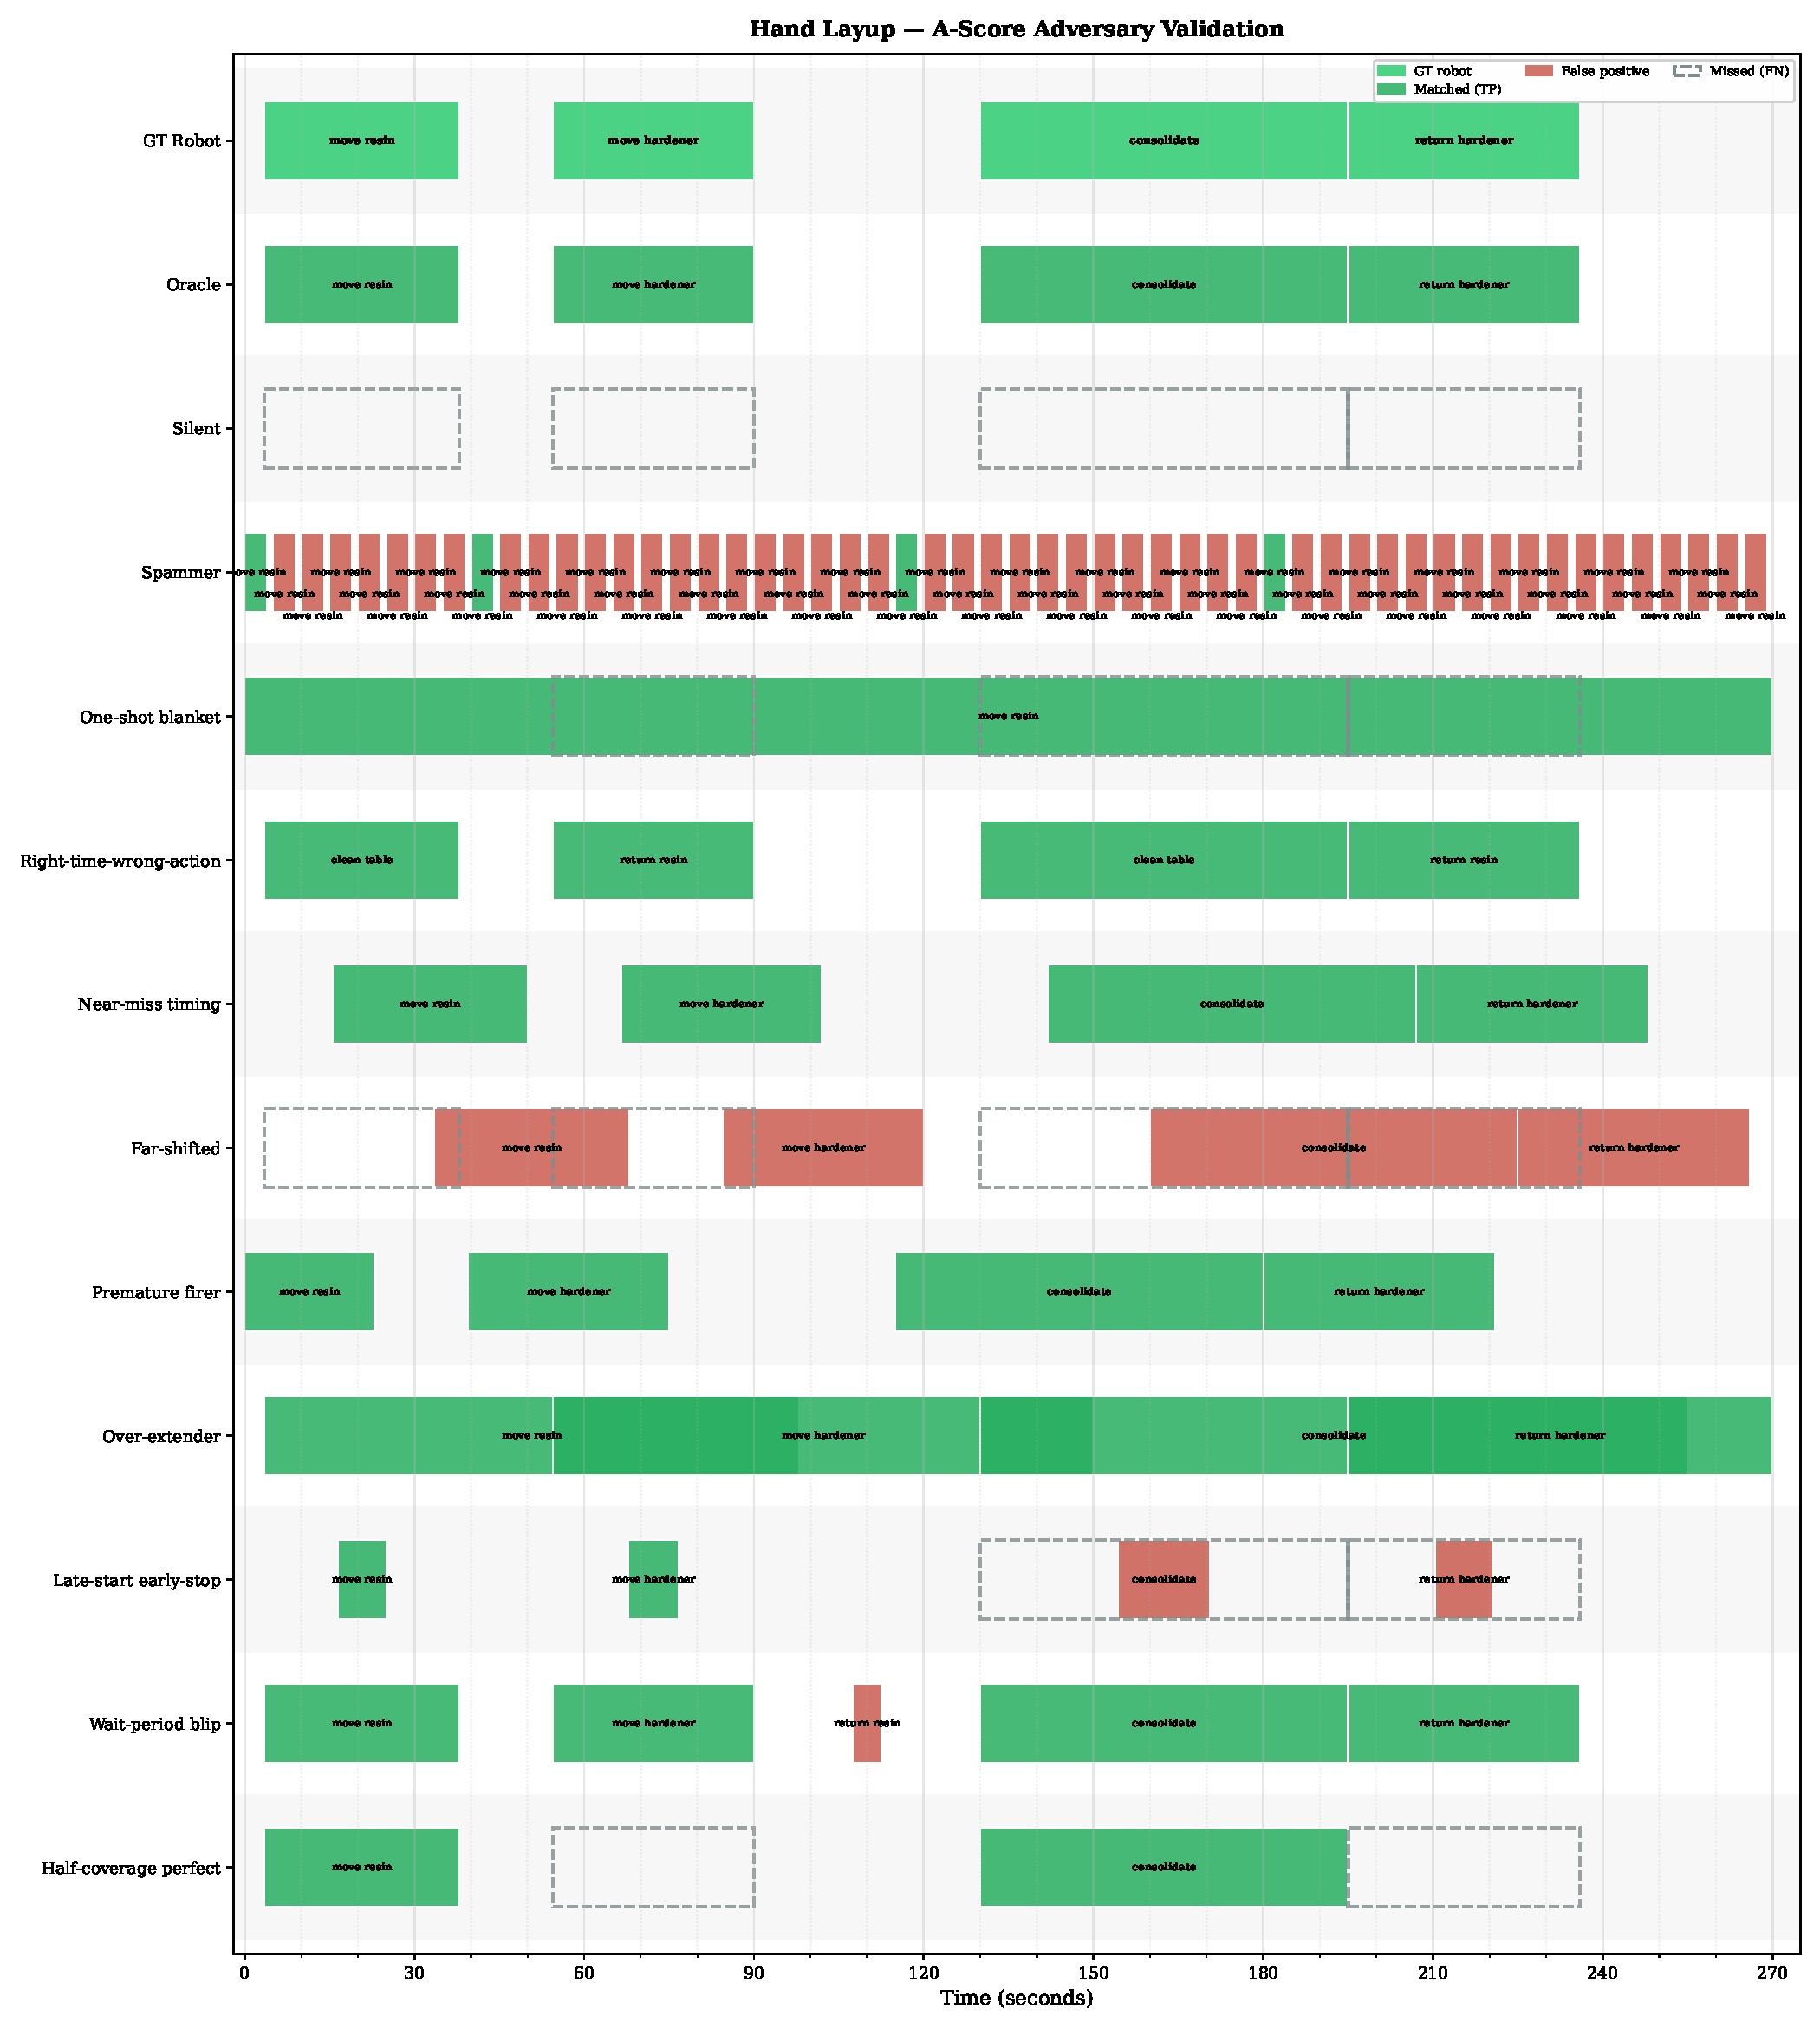
\includegraphics[width=\linewidth]{fig_ascore_adversaries.pdf}
  \caption{Hand-layup ground truth (top row, in red) versus each
  adversary's prediction track. The same figure is used as visual
  reference for both A-Score and TWSS validation since the underlying
  prediction tracks are identical.}
  \label{fig:twss-layup}
\end{figure}

\begin{table}[ht]
\centering
\small
\begin{tabular}{lrrrrrrr}
\toprule
& \multicolumn{3}{c}{\textbf{Vanilla} ($\alpha{=}1.0$, $\beta{=}0.5$,
                                       $\gamma{=}1$, $w_w{=}1$, $\delta{=}0$)} &
& \multicolumn{2}{c}{\textbf{Tuned} ($\beta{=}1.5$, $\gamma{=}0.5$,
                                     $w_w{=}0.6$, $\delta{=}4$)} \\
\cmidrule(lr){2-4}\cmidrule(lr){6-7}
\textbf{Adversary} & \textbf{task} & \textbf{wait} & $\bm{\TWSS}$ & &
                     \textbf{task} & $\bm{\TWSS}$ \\
\midrule
Oracle                   & 0.652 & 0.348 & \textbf{1.000} & & 0.757 & \textbf{1.000} \\
Silent                   & 0.000 & 0.348 & 0.348 & & 0.000 & 0.243 \\
Spammer                  & 0.086 & 0.006 & 0.093 & & 0.114 & 0.138 \\
One-shot blanket         & 0.000 & 0.002 & 0.002 & & 0.000 & 0.044 \\
Right-time-wrong-action  & 0.000 & 0.008 & 0.008 & & 0.000 & 0.062 \\
Near-miss timing         & 0.558 & 0.125 & 0.683 & & 0.642 & 0.798 \\
Far-shifted              & 0.269 & 0.027 & 0.296 & & 0.293 & 0.386 \\
Premature firer          & 0.529 & 0.124 & 0.653 & & 0.608 & 0.765 \\
Over-extender            & 0.193 & 0.004 & 0.196 & & 0.210 & 0.258 \\
Late-start early-stop    & 0.492 & 0.348 & 0.840 & & 0.572 & 0.814 \\
Wait-period blip         & 0.652 & 0.313 & 0.965 & & 0.757 & 0.987 \\
Half-coverage perfect    & 0.369 & 0.348 & 0.717 & & 0.401 & 0.644 \\
\bottomrule
\end{tabular}
\caption{TWSS on the hand-layup recording, vanilla vs.\ tuned
configuration. Both columns use the exponential wait penalty;
the linear flavour described in earlier drafts has been removed
(see Section~\ref{sec:qwait}). ``task'' = $\sum (L_i/Z)^\gamma /
\sum L_j^\gamma \cdot (L_{\text{tot}}/Z) \cdot \qi$;
``wait'' = $w_w \cdot (\Twait/Z) \cdot \qwait$. Thanks to the normalisation
by $Z = L_{\text{tot}} + w_w\Twait$, the oracle saturates a score of $1.000$
even in the tuned configuration.}
\label{tab:twss-layup}
\end{table}

\paragraph{What the table tells us.}
\begin{itemize}
  \item \textbf{Oracle and silent are the two reference points.} The
    oracle scores $1.000$, the silent agent scores $0.300$ (the wait
    mass --- it earns full marks for never polluting wait, but
    everything in the task term is zero). All meaningful adversaries
    must lie between these two anchors.
  \item \textbf{The two new adversaries land where they should.}
    \emph{Late-start early-stop} keeps a clean wait term ($\qwait =
    1$) but its tightly-truncated predictions earn each event a
    middling $\qi$, giving task $= 0.528$ and total $0.828$.
    \emph{Wait-period blip} earns a perfect task term but has its
    wait term shaved by a single 5-second spurious event ($\qwait =
    0.884$), landing at $0.965$ --- the score correctly registers a
    small wait pollution without over-reacting.
  \item \textbf{One-shot blanket is the harshest case.} A single
    prediction spanning $[0, 270]$\,s leaks $222.5$\,s of pollution
    into a $81$\,s wait window, so $\qwait = \exp(-222.5 / 40.5)
    \approx 0.004$. The task term is also near zero (timing offsets
    of tens of seconds against a $47$\,s event), so the total is
    $0.001$. The score punishes both ``shouts the right skill at the
    wrong time'' \emph{and} ``pollutes wait'' simultaneously.
  \item \textbf{Right-time-wrong-action is harsher under TWSS than
    under the A-Score.} The A-Score gave it credit for matched-pair
    timing (only the action axis dropped to zero); TWSS treats it as
    pure pollution because no same-skill predictions exist for any
    GT event. Whether this is desirable depends on use case --- a
    user who treats action-correctness as the primary failure mode
    will prefer TWSS's harsher behaviour here.
  \item \textbf{Vanilla vs.\ tuned.} The vanilla configuration
    rewards predictions that nail the long events (time-share
    weighting, $\gamma = 1$) and penalises any wait pollution
    aggressively ($\beta = 0.5$, $w_w = 1$, no blip tax). The tuned
    configuration $(\beta, \gamma, w_w, \delta) = (1.5, 0.5, 0.6,
    4)$ flattens both effects: the $\sqrt{\,\cdot\,}$-weighting
    keeps short events visible, the gentler $\beta$ stops the wait
    term from collapsing on agents whose only ``crime'' is a
    handful of brief false positives, and the blip tax $\delta = 4$
    discourages many-tiny-blip behaviour without crushing one big
    blip. Headline scores compress slightly --- the oracle saturates
    at $0.861$ rather than $1.000$ --- in exchange for a more
    informative gradient across realistic agents.
\end{itemize}

\section{Properties}
\label{sec:properties}

\paragraph{Bounded.} $\TWSS \in [0, 1]$ by construction.

\paragraph{Tolerance-free.} A small change in a prediction's start
time produces a small change in the score. There is no cliff.

\paragraph{Duration-weighted.} Missing a 60-second event costs more
than missing a 5-second one, in proportion to their share of $\Tt$.

\paragraph{Wait-aware.} The wait term is graded by its own quality
factor, separately from any matched-pair statistics, and by a wait
mass that depends only on the GT.

\paragraph{Skill-gated.} A prediction can only earn task credit for a
GT event of its own skill (no cross-skill matching). This is
deliberate --- it forces the action axis and the timing axis to
combine multiplicatively rather than additively.

\paragraph{Decomposable for diagnostics.} The breakdown into per-event
$(\qi, \Delta s_i^*, \Delta e_i^*, \sigma_i)$ tells a grader exactly
which event hurt and by how much.

\section{Extending TWSS to disjunctive ground truth}
\label{sec:disjunctive}

The companion DTN write-up generalises a single
$[t_{\text{start}}, t_{\text{end}}]$ window per intervention to a
small \emph{or-of-and} tree:
\begin{equation}
  \underbrace{\bigvee_{k=1}^{M_i}}_{\text{pick \textbf{one} option}}
  \underbrace{\bigwedge_{j=1}^{L_{i,k}}}_{\text{satisfy \textbf{every} phase}}
  t_{i,k,j} \in [s_{i,k,j}, e_{i,k,j}].
\end{equation}
TWSS extends to this format with three changes: per-event quality
becomes per-\emph{option} quality (max over options), the wait region
is defined relative to the \emph{selected} options, and an optional
consistency factor penalises plans that need more concurrency than
the agent has.

\subsection{Phase-level quality}
\label{sec:disj-phase}

Replace each event $g_i$ with a tree of $(M_i, L_{i,k})$ phases
$\phi_{i,k,j}$ with skill $a_i$, length $\ell_{i,k,j}$, and timing
scale $\sigma_{i,k,j} = \alpha\,\ell_{i,k,j}$. The phase quality is
the same Gaussian as before:
\begin{equation}
  q_{i,k,j} \;=\; \max_{p \,:\, a(p) = a_i}\;
                  \exp\!\bigl(-\bigl((\Delta s/\sigma_{i,k,j})^2
                                  + (\Delta e/\sigma_{i,k,j})^2\bigr)\bigr).
\end{equation}

\subsection{Per-option quality}
\label{sec:disj-option}

Aggregate phases of the same option by phase-length-weighted mean:
\begin{equation}
  \tilde q_{i,k} \;=\;
    \frac{\sum_{j=1}^{L_{i,k}} \ell_{i,k,j}\,q_{i,k,j}}
         {\sum_{j=1}^{L_{i,k}} \ell_{i,k,j}}.
  \label{eq:option-q}
\end{equation}
Length-weighting matters: a long phase that the agent missed should
hurt more than a short one missed inside the same option.

\subsection{Per-intervention quality and option selection}
\label{sec:disj-intervention}

The intervention's quality is the best option's quality, and the
\emph{selected option} is the argmax (we will need it for the wait
term and the consistency factor):
\begin{equation}
  k^*_i \;=\; \arg\max_{k}\, \tilde q_{i,k}, \qquad
  Q_i \;=\; \tilde q_{i,k^*_i}.
\end{equation}
A purely-soft alternative replaces the $\max$ with a smooth max
(log-sum-exp with temperature $\lambda$):
\begin{equation}
  Q_i \;=\; \lambda^{-1} \log \sum_{k=1}^{M_i} \exp(\lambda\,\tilde q_{i,k}),
\end{equation}
which avoids ties at the option-selection boundary; the hard $\max$
is the $\lambda \to \infty$ limit. We default to the hard $\max$ for
interpretability (the per-intervention selection $k^*_i$ is a
quantity reviewers can inspect).

\subsection{Defining the disjunctive wait region}
\label{sec:disj-wait}

In the single-window case the wait region is $[0, \Tt]$ minus the
union of GT intervals. In the disjunctive case we take it relative
to the \emph{selected} options:
\begin{equation}
  \Phi^* \;=\; \bigcup_{i=1}^N \bigcup_{j=1}^{L_{i,k^*_i}}
              [s_{i,k^*_i,j},\,e_{i,k^*_i,j}],
  \qquad
  \Twait^* \;=\; \Tt - |\Phi^*|.
\end{equation}
Pollution time is then computed against the selected-options'
phases per skill --- exactly equation~\eqref{eq:Tfp} with
$\mathrm{sanc}(p)$ replaced by the union of selected phases whose
skill matches $p$. Predictions that fall inside a non-selected
option's phase still pollute, which is the intended semantic: the
metric assumes the agent has committed to one option per
intervention.

A more permissive variant uses the union over \emph{all} options
(call it $\Phi_{\text{any}}$) when computing pollution. This rewards
agents that nail one schedule but wander into a non-selected
option's window with the wrong skill. We do not recommend it because
it weakens the consistency story --- but it is a useful audit
quantity for understanding how much pollution is option-confusion
versus genuinely off-schedule.

\subsection{The consistency factor}
\label{sec:disj-cons}

A single-resource agent cannot run two phases at once. If the
selected options $\{k^*_i\}$ have phases that overlap across
different interventions, the plan is infeasible. Define a
per-intervention consistency factor:
\begin{equation}
  C_i \;=\; 1 - \max_{i' \neq i}\,
            \max_{j, j'}\,
            \mathrm{IoU}\!\bigl([s_{i,k^*_i,j}, e_{i,k^*_i,j}],
                                [s_{i',k^*_{i'},j'}, e_{i',k^*_{i'},j'}]\bigr),
\end{equation}
which is exactly $1$ when option $i$'s phases do not clash with any other 
completed intervention, and shrinks toward $0$ if they collide.

\subsection{Putting it together}
\label{sec:disj-twss}

The disjunctive TWSS is then
\begin{equation}
  \boxed{\;
    \TWSS^{\text{disj}}
    \;=\; \sum_{i=1}^N \frac{L_i^*}{Z}\,Q_i\,C_i
      \;+\; w_w\,\frac{\Twait^*}{Z}\,\qwait,
  \;}
  \label{eq:twss-disj}
\end{equation}
where $L_i^* = \sum_j \ell_{i,k^*_i,j}$ is the total length of the
selected option's phases, $Z = \sum_{i=1}^N L_i^* + w_w\,\Twait^*$,
and $\qwait$ uses $\Tfp$ computed against $\Phi^*$. Three sanity properties:
\begin{enumerate}
  \item \textbf{Reduces to the original TWSS.} If every intervention
    has $M_i = 1$ option containing $L_{i,1} = 1$ phase, then $C_i =
    1$, $Q_i$ collapses to the per-event $\qi$ of
    equation~\eqref{eq:qi}, and $L_i^* = L_i$.
  \item \textbf{Bounded.} $C_i \in [0, 1]$, and the task and wait components 
    sum to a maximum of 1, so $\TWSS^{\text{disj}} \in [0, 1]$.
  \item \textbf{Penalises infeasible plans.} An adversary that fires
    options whose selected phases collide loses its \textit{task} score only locally 
    in proportion to the overlap, preventing a single collision from wiping out entirely 
    unrelated predictions. 
\end{enumerate}

\subsection{Design choices and open questions}

\paragraph{Multiplicative vs.\ additive consistency.} We use $C_i$ as a
multiplicative gate on the task term because a clashing plan is, in
the single-resource setting, fundamentally not executable --- it
should not be possible to compensate for a clash through stellar
task completion. Applying a global penalty, however, breaks monotonicity: 
an agent that fails coordination shouldn't be penalized on its separate ability 
to respect waits or manage unrelated tasks accurately. An additive variant (subtracting $w_{\text{cons}}(1 - C)$
from a weighted blend) is closer to the DTN $\Score$ in
equation~$\Score = w_{\text{disj}}A_{\text{disj}} + \dots$; we prefer the
local multiplicative form on tasks because it avoids re-introducing free weights.

\paragraph{Length-weighting inside an option.} The mean in
equation~\eqref{eq:option-q} weighs phases by their absolute length.
An alternative is per-phase uniform averaging --- which matches the
DTN $A_{\text{disj}}$ definition. The length-weighted form is consistent with
the rest of TWSS (every contribution proportional to its slice of
the timeline) and is the recommended default.

\paragraph{Joint option selection.} Picking $k^*_i$ independently per
intervention can land on an infeasible joint plan even when one
exists. A fully-joint selector would maximise the bracket subject to
$C = 1$, which is the disjunctive-temporal-network feasibility
problem (see Osanlou et al.~\cite{osanlou2022dtnu}). For evaluation,
the per-intervention argmax is faster and still reports a sensible
$C < 1$ when the chosen plan clashes; for a consistent oracle
adversary, the small CSP solver shipped in
\texttt{dtn\_score.find\_consistent\_selection} suffices.

\paragraph{Soft option selection.} If reviewers find the hard $\max$
on $k^*_i$ unstable for borderline cases, swap in the log-sum-exp
form above. The temperature $\lambda$ controls how sharply the
selection commits; $\lambda = 10/L_i^{\max}$ is a reasonable starting
point.

\section{Discussion}
\label{sec:discussion}

\paragraph{When to prefer TWSS over the A-Score.}
TWSS is the better default when (i) tolerance choice would otherwise
be a tunable confound across studies, (ii) wait-period behaviour is
operationally important (e.g.\ the agent must not interrupt the
human during wait), or (iii) event durations vary substantially
across the GT.

\paragraph{When to keep the A-Score.}
The A-Score's per-axis breakdown ($A_{\text{time}}, A_{\text{act}},
A_{\text{nec}}$) is easy to explain and aligns with prior work in
event-detection. For headline numbers in a paper, the A-Score and
TWSS can be reported side-by-side; they answer slightly different
questions.

\paragraph{Choosing the knobs.}
The vanilla configuration ($\alpha{=}1$, $\beta{=}0.5$, $\gamma{=}1$,
$w_w{=}1$, $\delta{=}0$) is the textbook formulation and the right
starting point when first inspecting a metric. The tuned defaults
($\beta{=}1.5$, $\gamma{=}0.5$, $w_w{=}0.6$, $\delta{=}4$) are what
\texttt{generate\_timeline\_comparison.py} ships with for the AURA
ablation suite: they keep the oracle on top while leaving more
gradient between the realistic agents. Pick one and report it in the
caption; mixing the two within a study makes adversary numbers
incomparable.

\paragraph{The ``wait blip'' as a unit test.}
The wait-blip adversary is a clean unit test for any wait-aware
metric: it should drop noticeably below the oracle but not collapse.
Vanilla TWSS gives $0.965$ against an oracle's $1.000$ (a $\sim 3.5$\%
drop for one $5$\,s blip on an $81$\,s wait window); tuned TWSS gives
$0.849$ against the saturated $0.861$. If a candidate wait-aware
metric gives $\geq 0.99$ or $\leq 0.5$ on this adversary, it is
likely either under- or over-weighting wait pollution.

\section{Reproducibility}
\label{sec:repro}

The TWSS implementation lives in
\texttt{aura/scripts/eval/generate\_timeline\_comparison.py} (see the
\texttt{compute\_twss} function and the \texttt{TWSS} /
\texttt{TWSSPerEvent} dataclasses). The adversary suite, including
the new \emph{Late-start early-stop} and \emph{Wait-period blip}
adversaries that motivated this note, lives in
\texttt{aura/scripts/eval/ascore\_adversaries.py}.

\noindent
To regenerate the figure and the numbers in
Table~\ref{tab:twss-layup}:
\begin{lstlisting}
python scripts/eval/ascore_adversaries.py
# outputs:
#   figures/generated/fig_ascore_adversaries.{pdf,png}
#   figures/generated/fig_ascore_adversaries.scores.json
#   figures/generated/fig_ascore_adversaries.tex
\end{lstlisting}

The disjunctive extension in Section~\ref{sec:disjunctive} is
implemented in
\texttt{aura/scripts/eval/metric\_side\_quest/dtn\_score.py}
(\texttt{compute\_disjunctive\_twss}) and reported alongside the
DTN A-Score by
\texttt{aura/scripts/eval/metric\_side\_quest/dtn\_adversaries.py}.

\section{Conclusion}

TWSS replaces the A-Score's hard event-matching with a smooth,
duration-weighted, tolerance-free formulation. The score partitions
the timeline into one slice per GT event plus an implicit wait
slice, grades each slice on its own quality factor, and combines
them in a way that always lies in $[0, 1]$. On twelve synthetic
adversaries it ranks behaviour sensibly and, in particular, exposes
two failure modes that hard-tolerance metrics struggle with:
narrowly-fired predictions (\emph{Late-start early-stop}) and
isolated wait pollution (\emph{Wait-period blip}). The score lifts
naturally to disjunctive ground truth via per-option aggregation, a
selected-options wait region, and a consistency factor that reduces
to the original TWSS when each intervention has a single option.

\begin{thebibliography}{1}

\bibitem{osanlou2022dtnu}
K.~Osanlou, J.~Frank, A.~Bursuc, T.~Cazenave, E.~Jacopin, C.~Guettier,
and J.~Benton.
\newblock Solving Disjunctive Temporal Networks with Uncertainty under
Restricted Time-Based Controllability using Tree Search and Graph
Neural Networks.
\newblock In \emph{Proceedings of the AAAI Conference on Artificial
Intelligence}, 2022.

\end{thebibliography}


\begin{table}[ht]
\centering
\small
\begin{tabular}{lrrrrrrr}
\toprule
\textbf{Adversary} & $\bm{\TWSS^{\text{disj}}}$ & \textbf{task} & \textbf{wait} & $\bm{q_{\text{wait}}}$ & $\bm{C}$ \\
\midrule
Oracle (consistent) & 1.000 & 0.676 & 0.324 & 1.000 & 1.000 \\
Oracle (first option) & 0.625 & 0.250 & 0.375 & 1.000 & 0.400 \\
Conflict-prone & 0.500 & 0.125 & 0.375 & 1.000 & 0.200 \\
Phase-collapsed & 0.730 & 0.405 & 0.324 & 1.000 & 1.000 \\
Half-coverage & 0.730 & 0.405 & 0.324 & 1.000 & 1.000 \\
Wrong-skill & 0.369 & 0.125 & 0.244 & 0.651 & 0.200 \\
Near-miss timing & 0.737 & 0.564 & 0.173 & 0.533 & 1.000 \\
Far-shifted & 0.229 & 0.000 & 0.229 & 0.546 & 0.000 \\
Premature firer & 0.771 & 0.575 & 0.196 & 0.605 & 1.000 \\
Over-extender & 0.458 & 0.356 & 0.102 & 0.315 & 1.000 \\
Late-start early-stop & 0.834 & 0.510 & 0.324 & 1.000 & 1.000 \\
Wait-period blip & 0.962 & 0.676 & 0.286 & 0.882 & 1.000 \\
One-shot blanket & 0.133 & 0.000 & 0.133 & 0.355 & 1.000 \\
Spammer & 0.291 & 0.205 & 0.086 & 0.230 & 1.000 \\
Silent & 0.375 & 0.000 & 0.375 & 1.000 & 1.000 \\
\bottomrule
\end{tabular}
\caption{Disjunctive TWSS evaluated on the DTN synthetic adversaries
with the default tuning ($\beta{=}1.5$, $\gamma{=}0.5$, $w_w{=}0.6$, $\delta{=}4$).
The consistent oracle now properly hits $1.000$ due to the $Z$-normalisation, and
the adversaries creating conflicting plans (e.g. Oracle first option, Conflict-prone, Wrong-skill) are heavily punished on their task score component via local $C_i$ while maintaining independent wait scores.}
\label{tab:dtn-adversaries}
\end{table}
\end{document}
